\subsection{Runtime view}
In this section, to clarify better how the system works dynamically at runtime, a series of sequence diagram is shown:
\begin{itemize}
\item Log-in diagram
\item Request-acceptance diagram
\item Publish group request diagram
\item Automated SOS call diagram
\item Close race diagram
\item Send cluster of data diagram
\end{itemize}

\subsubsection{Log-in sequence diagram}
The log in is an important feature of large interest, because it is also central for the process of handling the users' session. The next
diagram exposes the procedure for the user.

\begin{figure}[H]
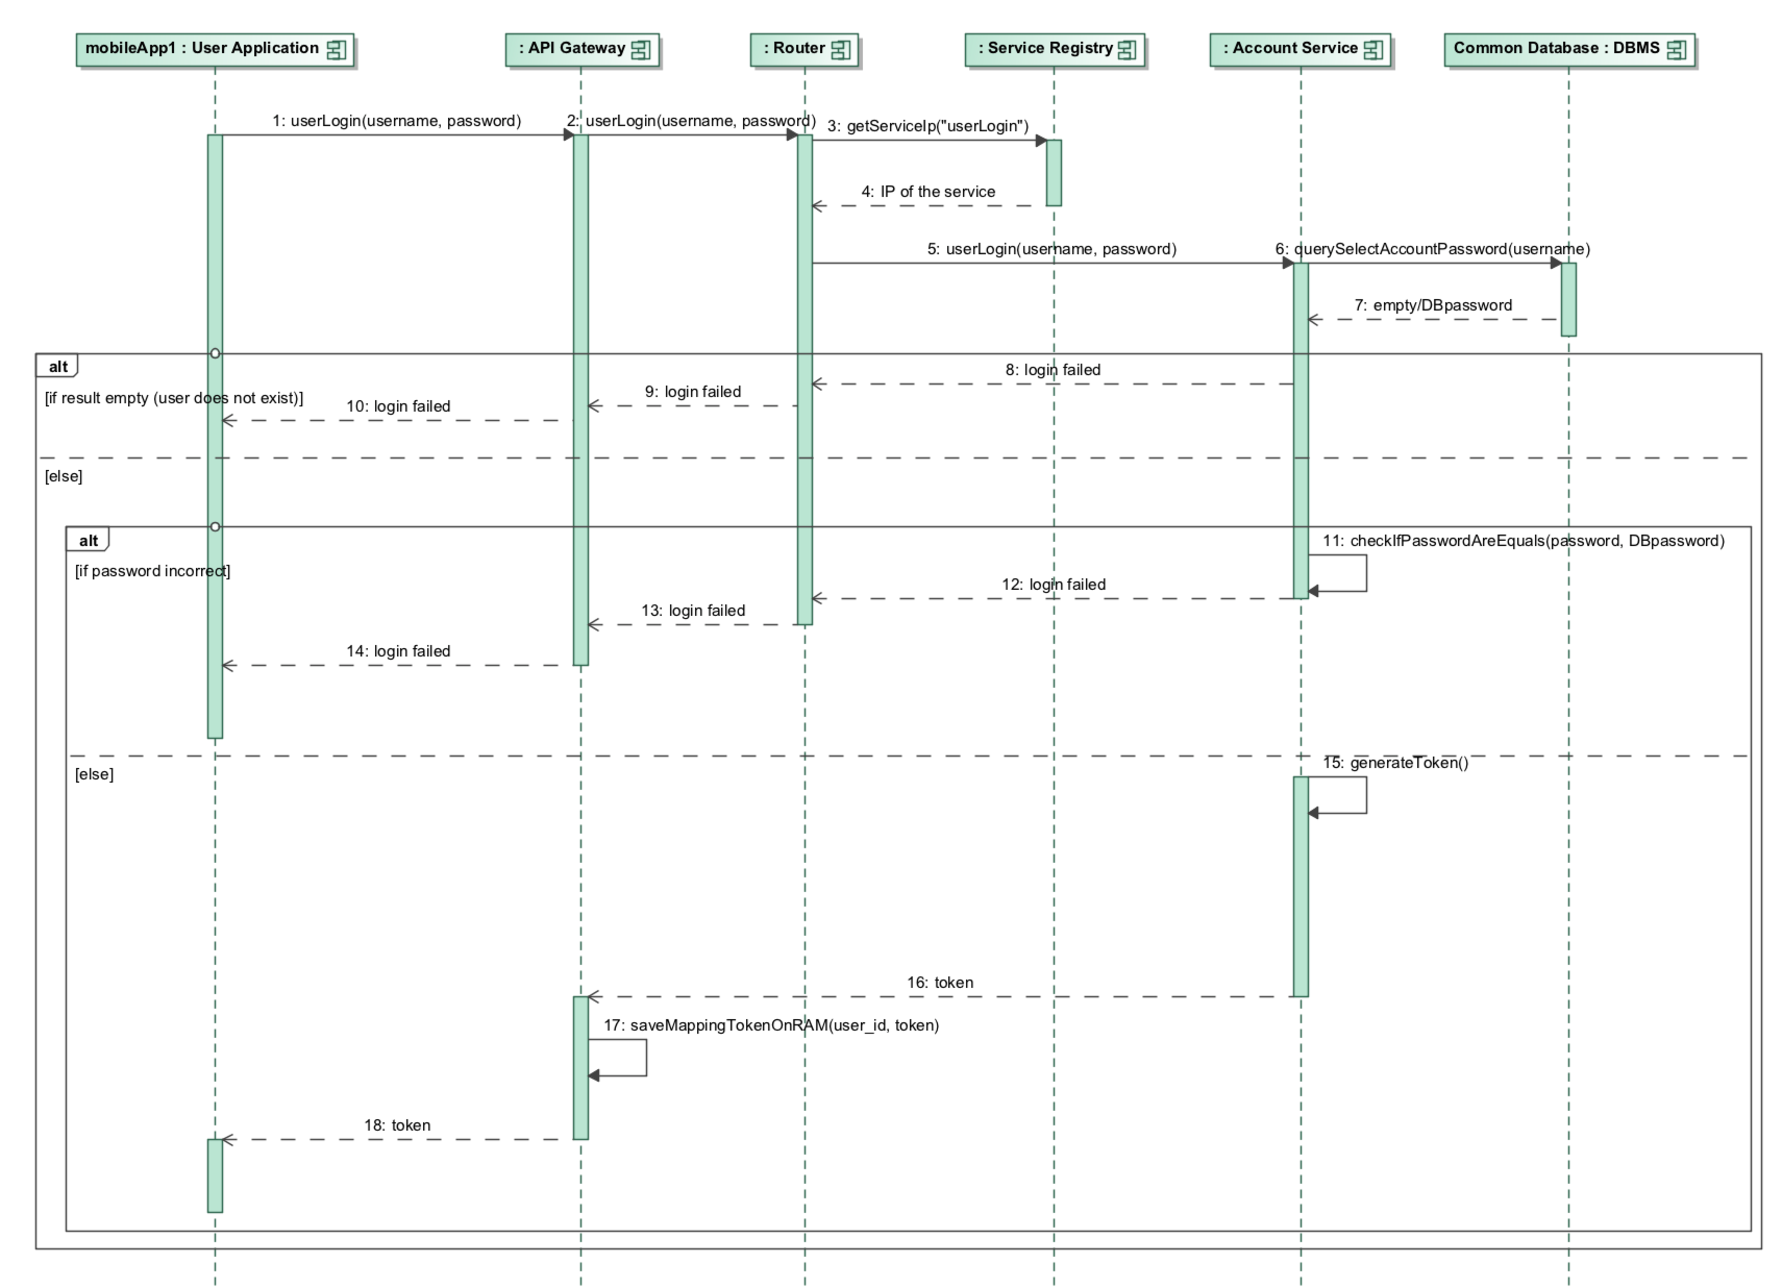
\includegraphics[width=\linewidth]{Images/login.pdf}
\caption{ Sequence diagram: log in}
\label{fig:login}
\end{figure}

Only in this diagram, it is shown how the router and service registry works when they are called from the API gateway due to achieve simplicity on other diagrams which are more complex. As the diagram show, if the log-in is done correctly, a token is generated from the account service and returned back to the API gateway
and to the client. 
The information will be used by both the client and the API gateway to manage the user session: all the next requests will be authenticated
using that token.  \\

\subsubsection{Request-acceptance sequence diagram}
An important issue in the project is the process in which the user gives a reply to an individual request
performed by a third party customer. 
This is exploited in the following diagram, that assumes that the user
is already logged in and that the list of pending request is non-empty.
\begin{figure}[H]
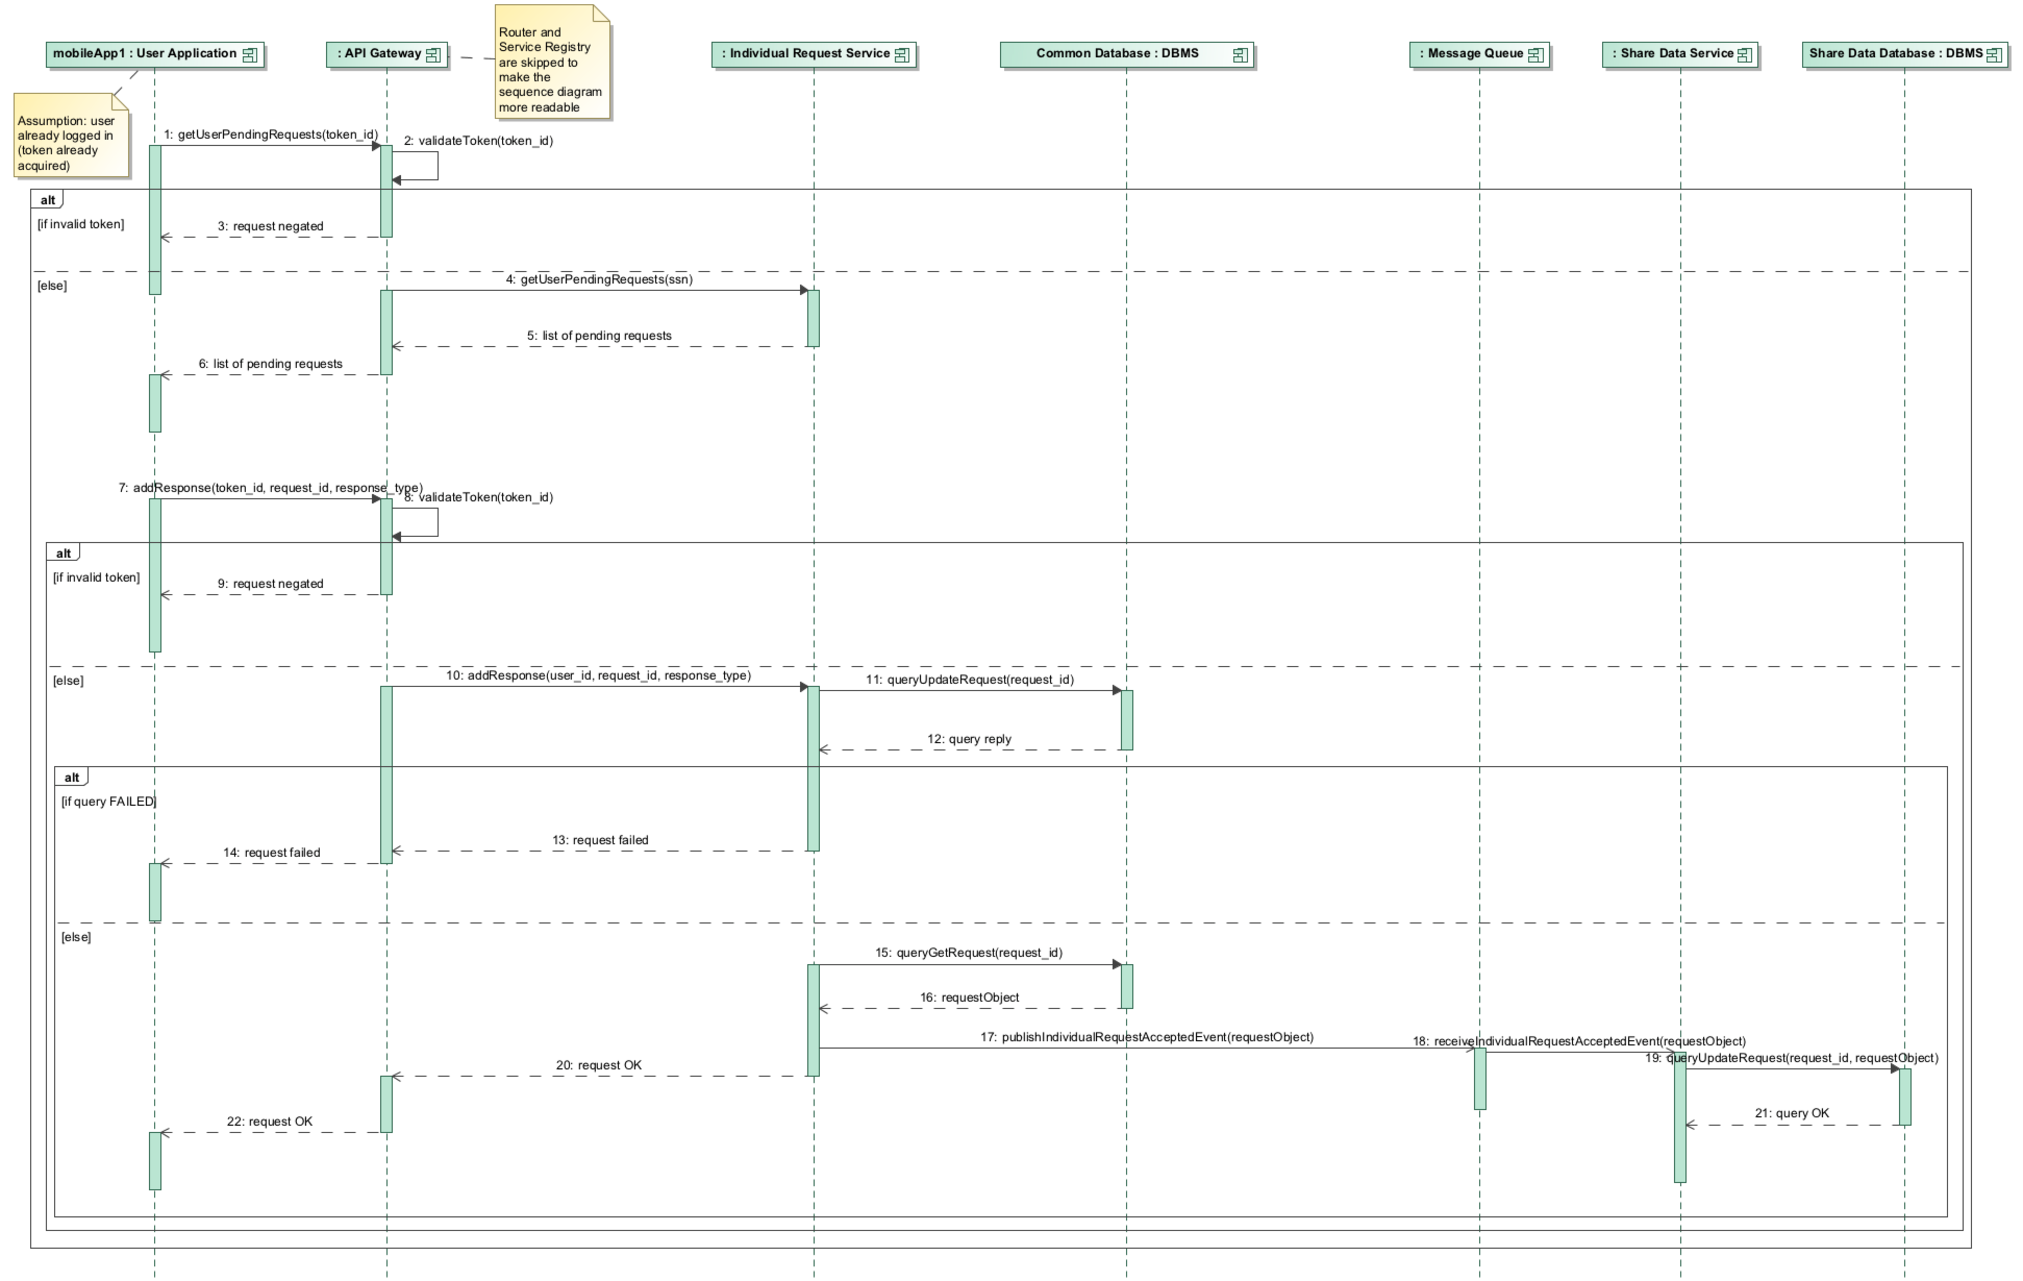
\includegraphics[width=\linewidth]{Images/requestacceptance.pdf}
\caption{ Sequence diagram: request acceptance }
\label{fig:requestacceptance}
\end{figure}

Some comments follows in order to clarify some essential points:
\begin{itemize}
\item The API gateway functions also as a proxy for the authentication service. In particular, it keeps track of the active sessions of the
users (identified by a token\_id). This information is in memory since
it was returned from the account service in the moment in which that user has performed the log-in
\item The communication between services is kept asynchronous, in order to reduce the response time 
toward the user that initially used the individual request service. This is acceptable because there are
no strict requirement on the efficiency on the access of data by third party customer (i.e. the data should
not be available in the exact moment in which an user sends a response: some latency is tolerated). 
\item The share data service needs information about requests that have been accepted, in order to correctly
provide the data access in the right way (i.e. granting access if an accepted request on the data has been 
accepted). Therefore, when a request is assigned to a new status in the individual request service, this information is communicated
\item the Message Queue component is responsible to forward the event of new request status to all the other services which has subscribed to this event. This helps to achieve a messaging system able to send asynchronous messages across services.
\end{itemize}


\subsubsection{Publish group request sequence diagram}
Another important feature is the fact that third party customers can perform requests on aggregated data. \\


\begin{figure}[H]
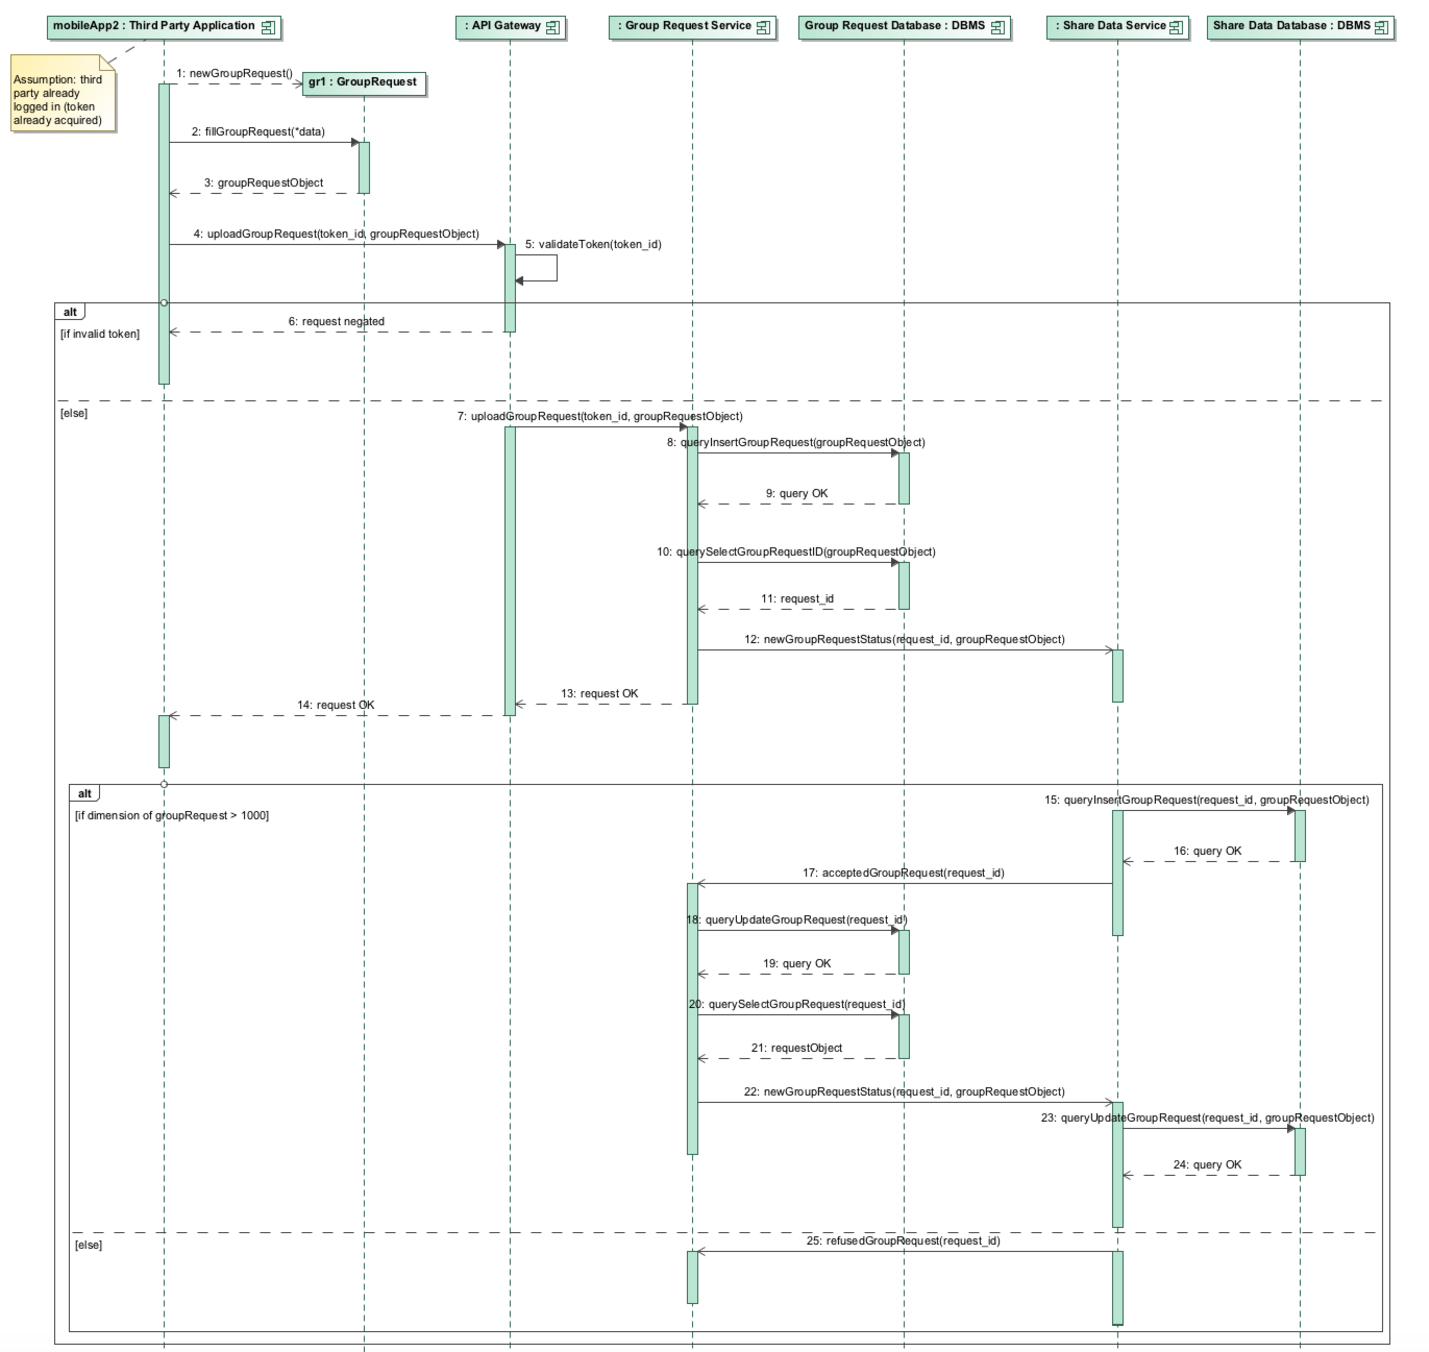
\includegraphics[width=\linewidth]{Images/grouprequest.pdf}
\caption{ Sequence diagram: group request }
\label{fig:grouprequest}
\end{figure}

The same comments of the previous diagram hold, also, in this situation. 
However, it is relevant to clarify the asynchronous exchange of messages that happens between the group request service and the share data
service. 
In the first place, it is necessary to point out that when a third party customer sends a group request, it is reasonable to assume that 
some time to serve and verify the request can be taken, but a non-desired behavior is to block the client in waiting the response. The status
of the request can be checked in a second moment, always via the group request service. 
Therefore, when a petitioner asks for some aggregated data, the group request service will delegate to the share data service the task of 
analyzing the request: it will then reply with the number of user involved. If this number is greater than 1000, the group request service
changes the status of the request from "in progress" to "accepted" and it will send this information to the share data service, that, thus,
will be able to provide correct access to the requested data. \\

\subsubsection{Automated SOS call sequence diagram}
Another critical feature of the project is the one regarding AutomatedSOS: 

\begin{figure}[H]
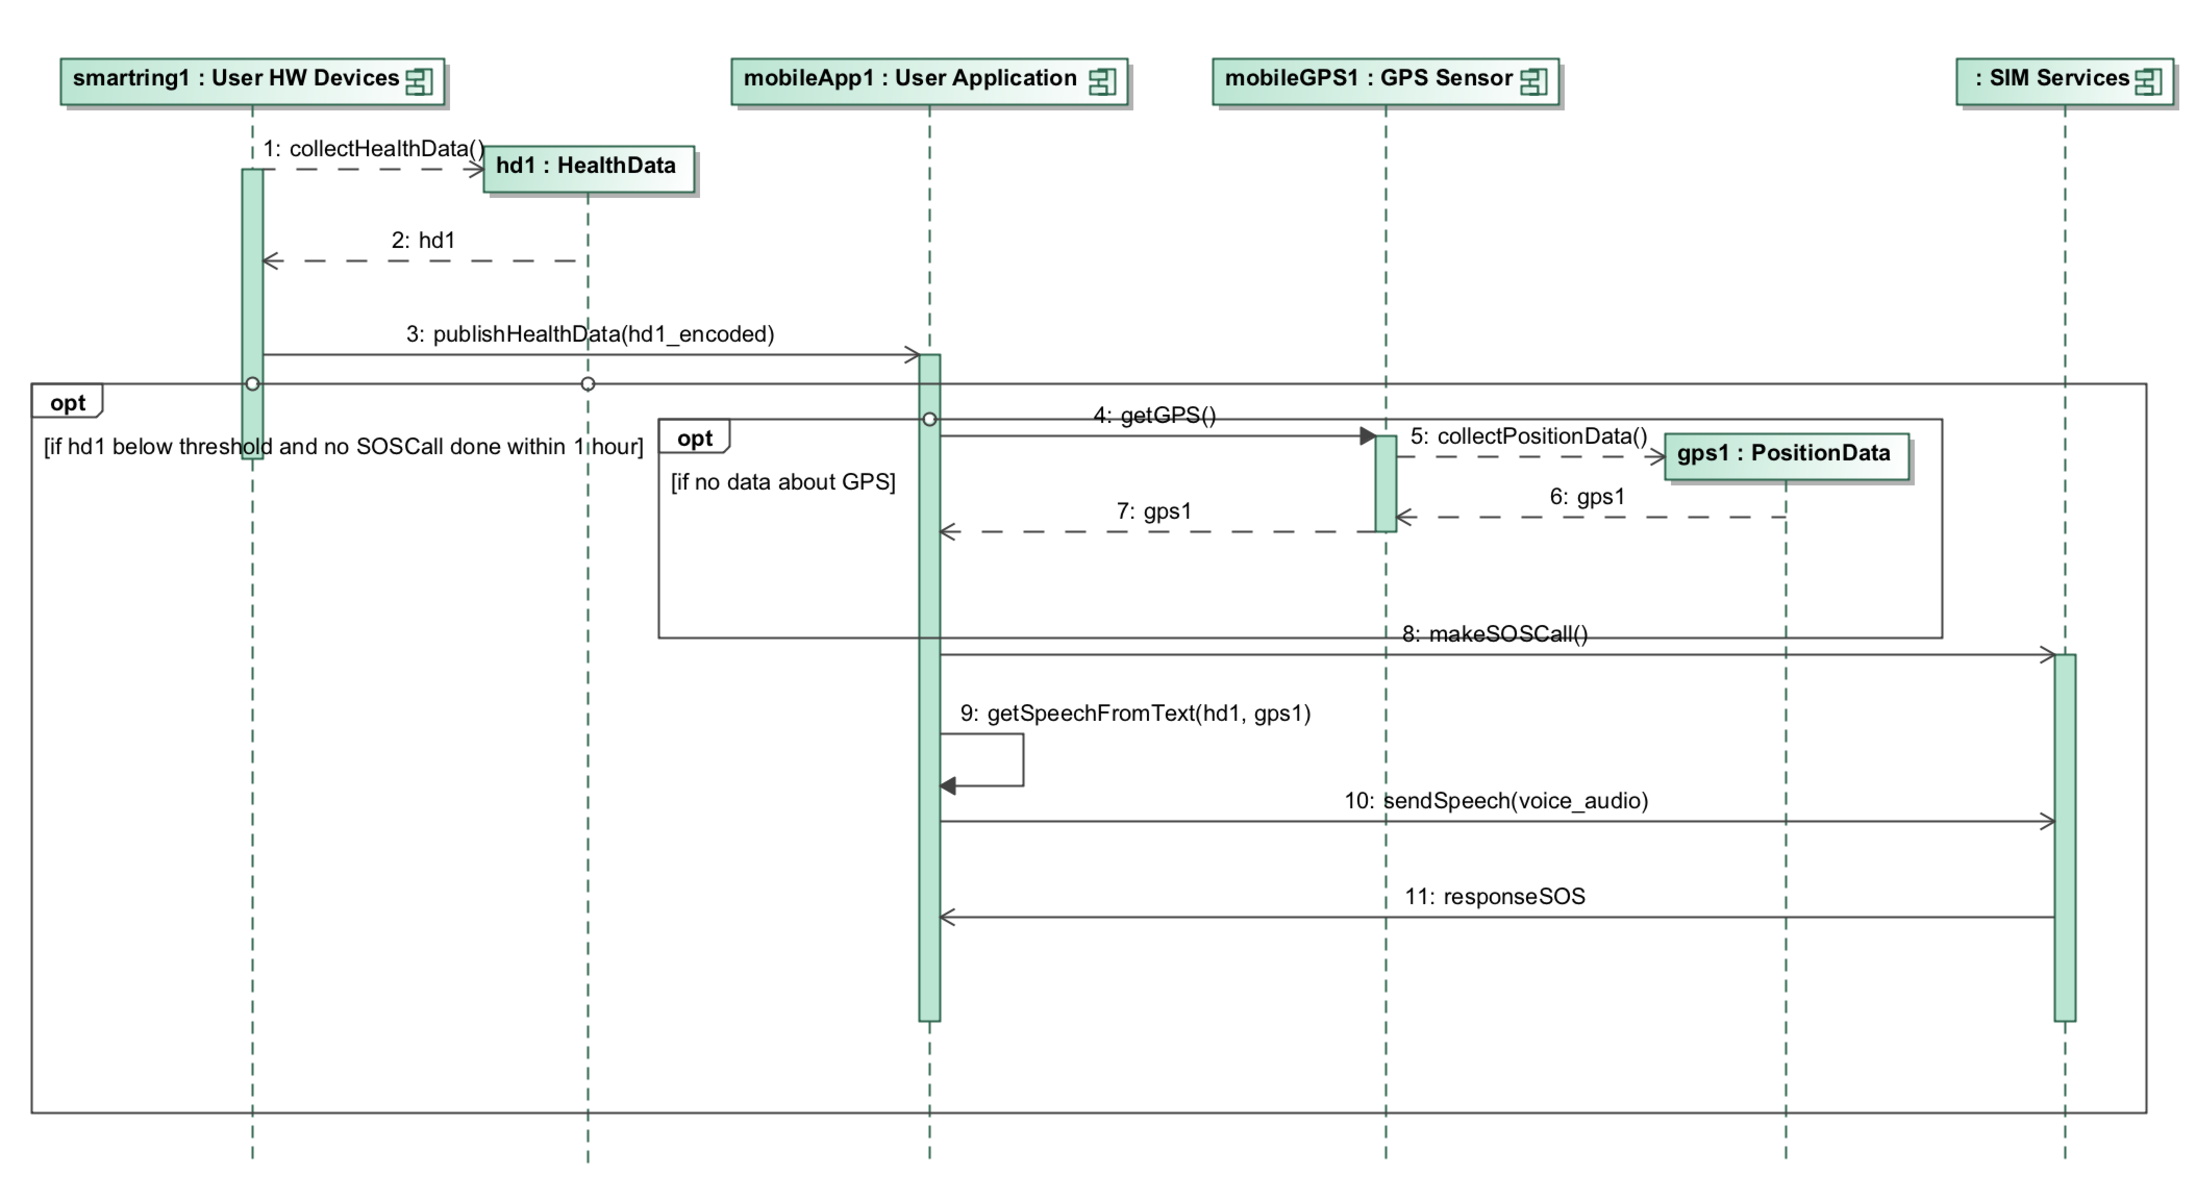
\includegraphics[width=\linewidth]{Images/automatedsos.pdf}
\caption{ Sequence diagram: automated SOS call}
\label{fig:automatedSOScall}
\end{figure}

This feature is implemented locally, in the mobile application, in order to guarantee the best efficiency and reduce to the minimum delays
that may be introduced due to data transfer over the Internet. 
Indeed, the diagram shows that the user hardware device component will collect user health data, and send them to the user application: if this observes some parameters below the threshold, it will perform an SOS call. 
The call is handled in the following way: the mobile app uses a default template to communicate with an emergency room operator all the
information needed to provide assistance (i.e. health data and position). 
The emergency room operator replies with a response that should be "Yes" or "No", in order that the application is aware of it.  \\

\subsubsection{Close race sequence diagram}
The procedure of closing a race is here described: 

\begin{figure}[H]
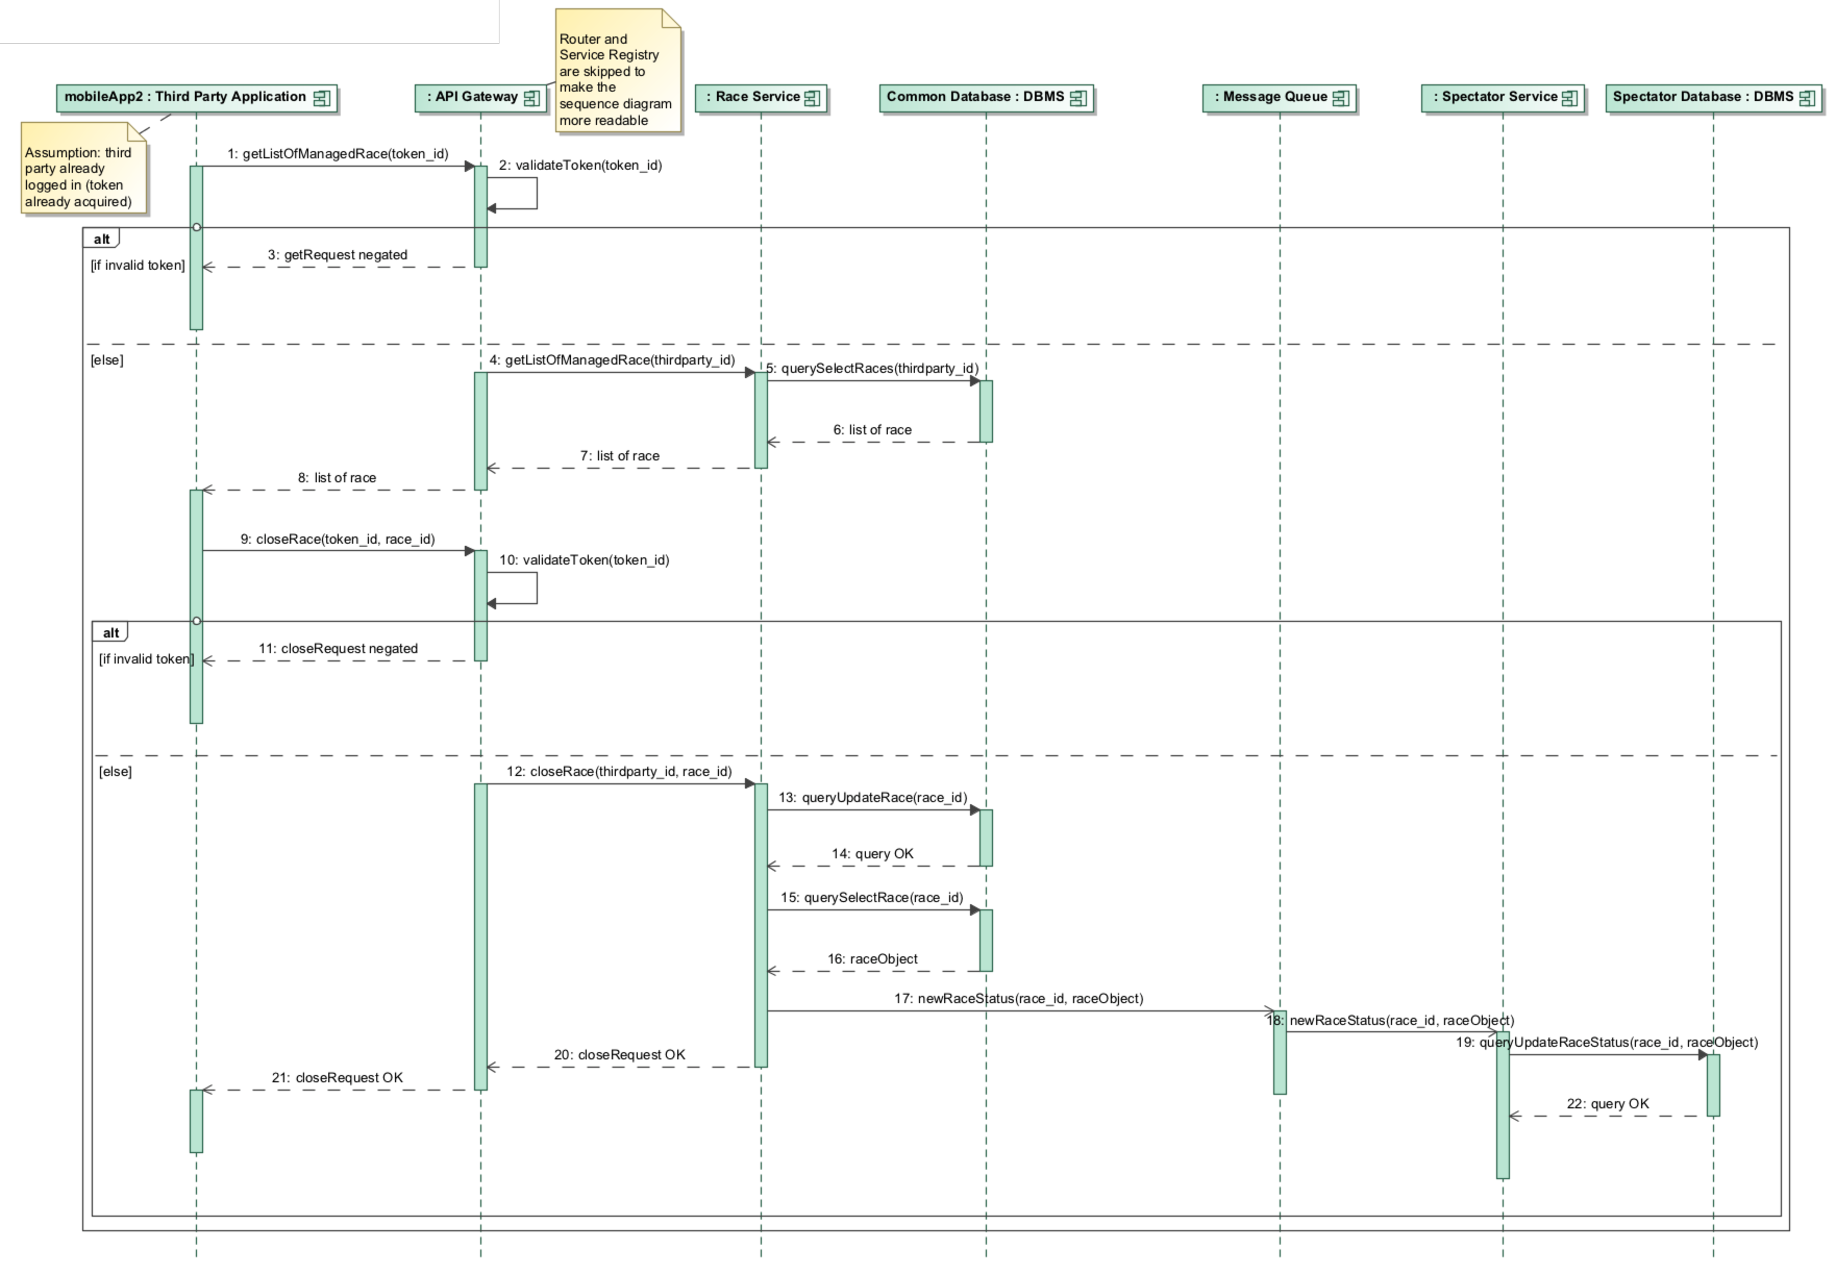
\includegraphics[width=\linewidth]{Images/closerace.pdf}
\caption{ Sequence diagram: close race}
\label{fig:closerace}
\end{figure}

It is worth to comment the asynchronous message from race service to spectator service. 
Indeed, in this case the race is successfully closed, therefore, data collection from athletes from that event should be stopped and not 
more available; and the same holds for the fact that users are no more able to see their positions, but only the leaderboard.
In order to accomplish this, an asynchronous call is here performed, to inform the spectator service. 
Note that some delay could happen, due to asynchronicity, in preventing the above mentioned features; however this is tolerated, because
it is not something considered that critical.

\subsubsection{Send cluster of data sequence diagram}
The interaction between components during the send of cluster of data done by a user is described as follows:

\begin{figure}[H]
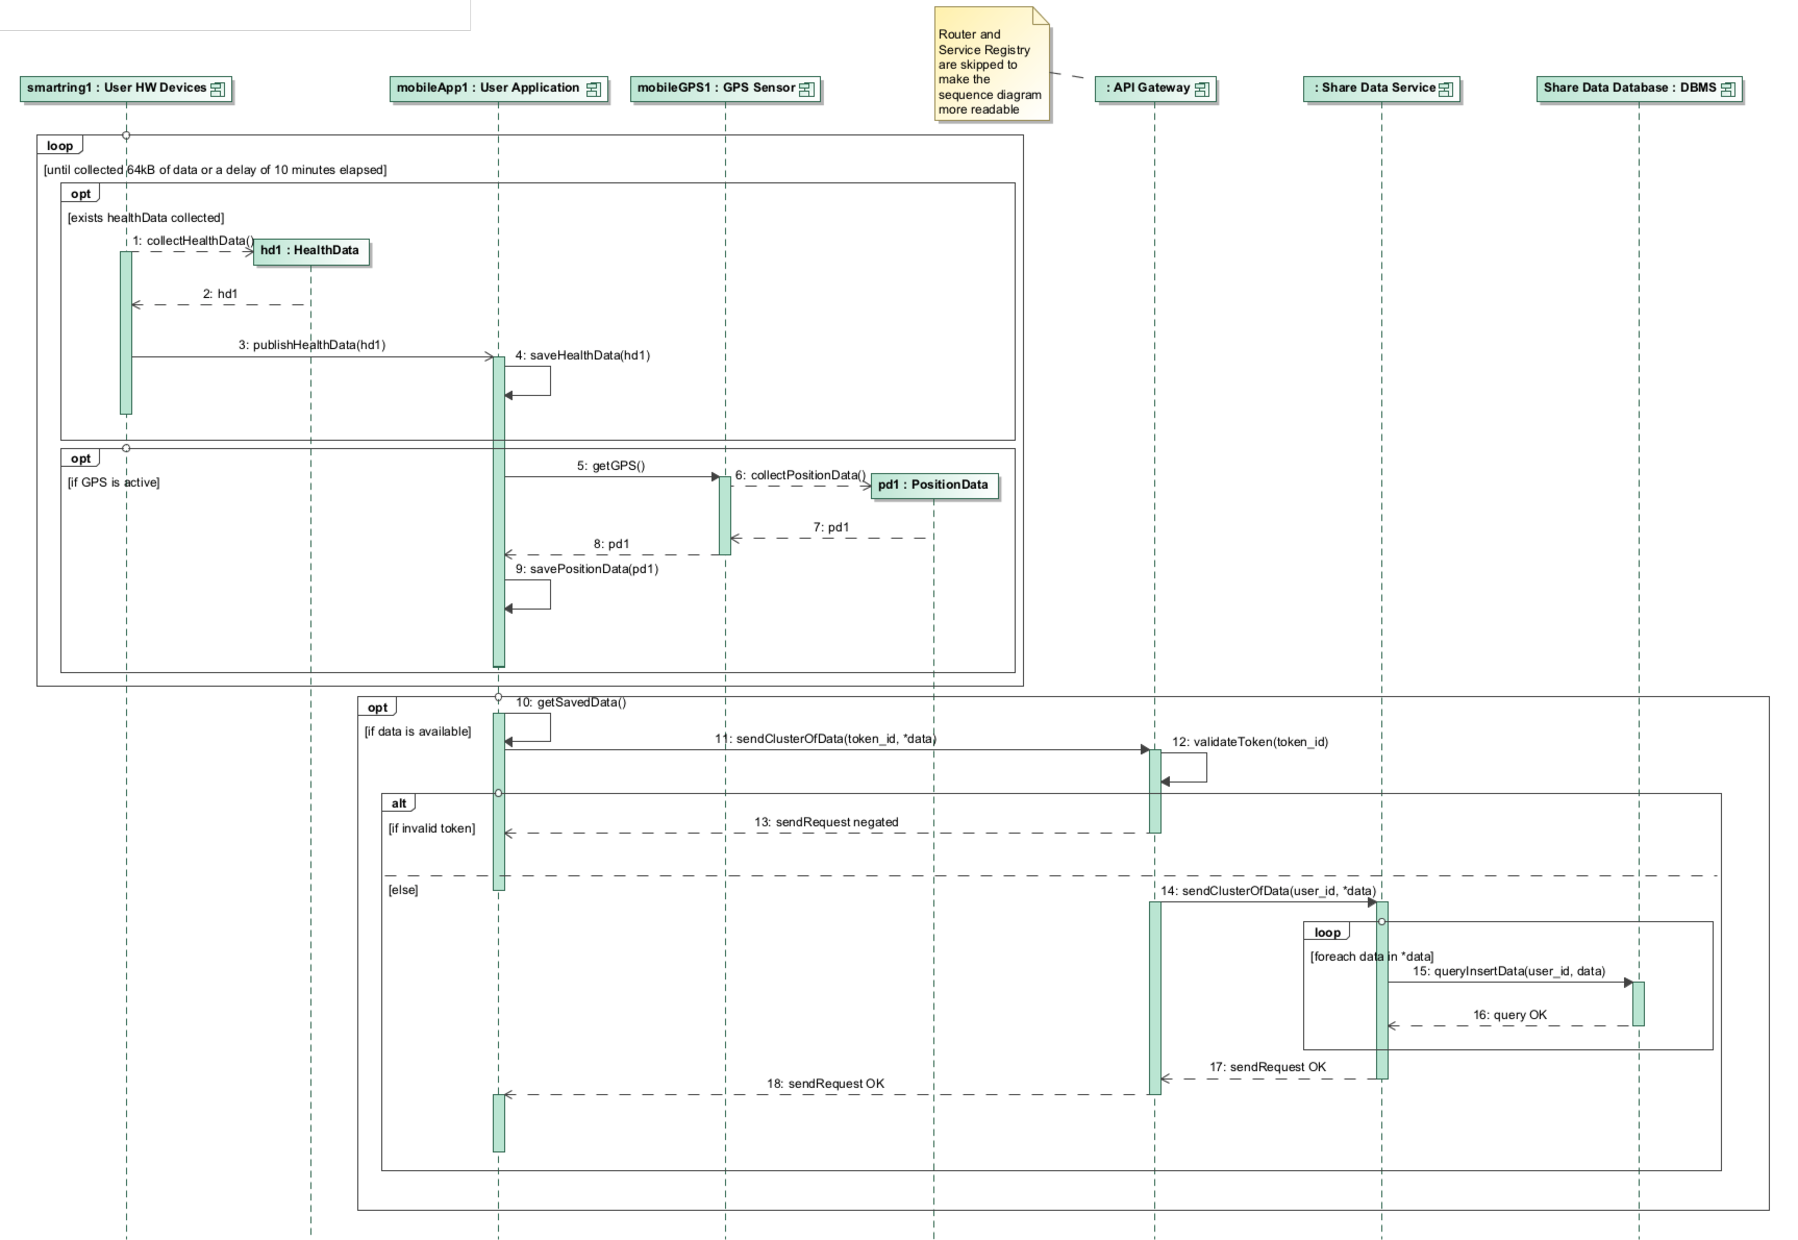
\includegraphics[width=\linewidth]{Images/senddata.pdf}
\caption{ Sequence diagram: send cluster of data}
\label{fig:closerace}
\end{figure}

The most of the request done by users is related to sending data to the TrackMe system. Therefore, this is one of the bottleneck 
of the system. By taking into consideration that more or less every application server accepts about 8kB of header HTTP request and the data to send at each time:
\begin{itemize}
\item token\_id: it is a token of 16 bytes, which is necessary to identify the user;
\item position data: it is, basically, two double representing latitude and longitude, but since the RESTful message cannot send double, it can be seen as two strings of 10 bytes;
\begin{figure}[H]
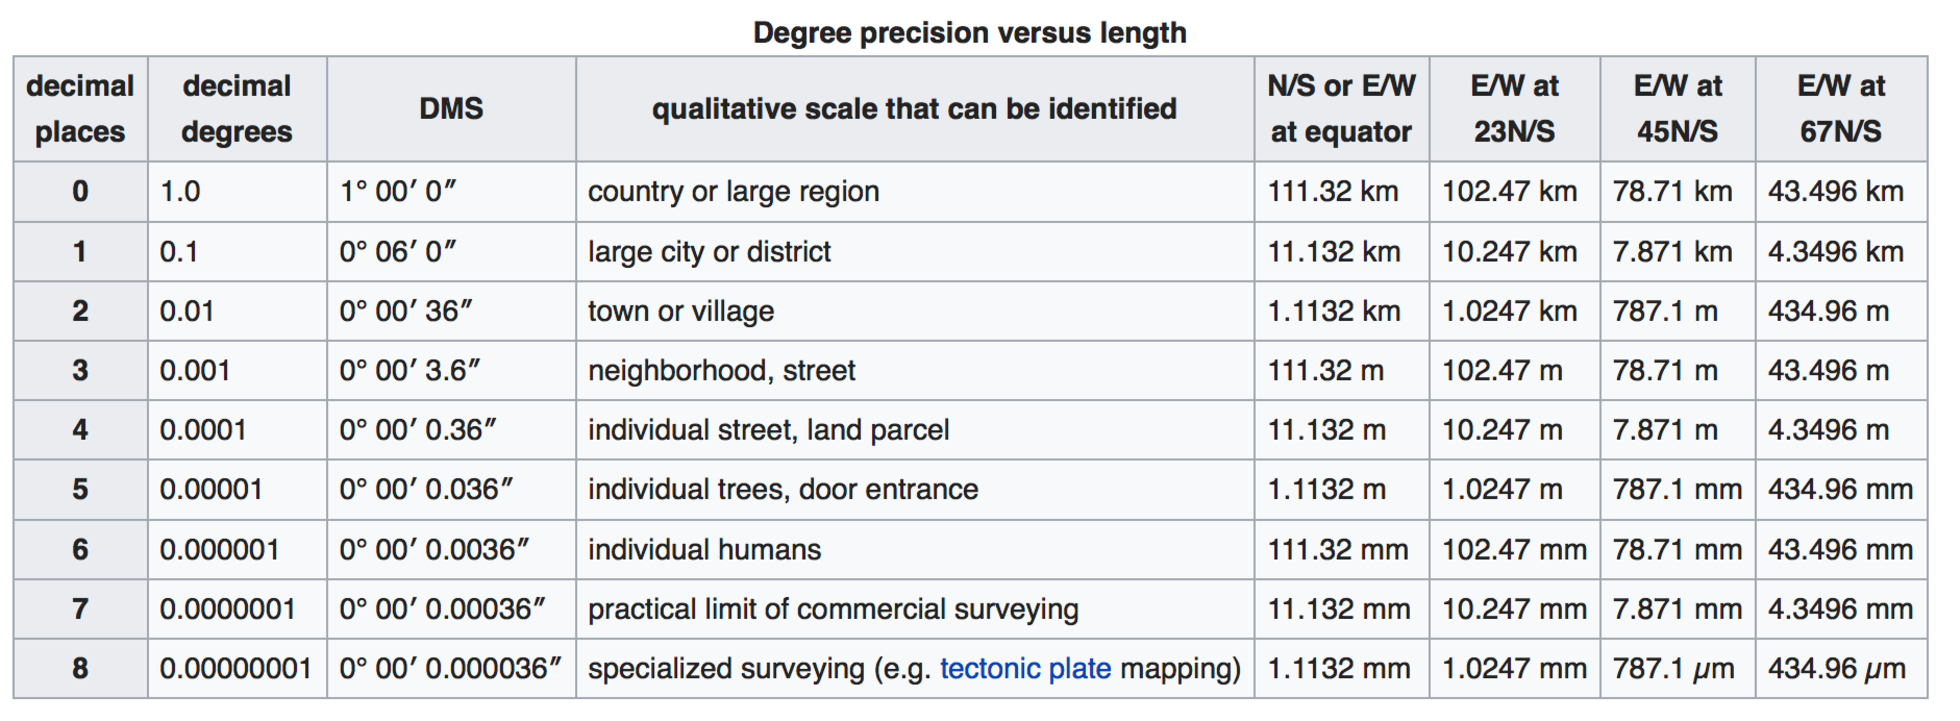
\includegraphics[width=\linewidth]{Images/gpsprecision.pdf}
\caption{ Degree precision versus length }
\label{fig:precisiongps}
\end{figure}
\item health data: this type of data can be a heartbeat value (i.e. integer), a blood pressure value (i.e. minimum pressure or maximum pressure, which means two integers), or a bloody oxygen level (i.e. integer). Therefore, at most it is possible to have 2 integers when a health data is sent.
\item timestamp: it usually weights 8 bytes when the timestamp has a timezone. To be coherent with everyone, the timestamp will always have a timezone of Greewich UTC.
\end{itemize}
Other than data, if the messages are, for instance, JSON they need a key which is a string. More or less a key can be estimated to be on average 10 bytes. Therefore, after this consideration, a possible recommendation about how periodically the user should send data is to do it once the data collected exceed 64 kB or when 10 minutes are elapsed. This choice is due to the fact that too much requests within a short time could overload the servers, but the system should also have updated data, so, if 10 minutes are elapsed from the last transfer and there are data available, then the user application should send data to TrackMe.
